
The $m_{lljj}$ ($m_{ZZ}$) distributions, depicted in Figure~\ref{fig:emuratios}
for the electron and muon channels, display an
excellent agreement both in the $m_{jj}$ sideband and signal regions.

\begin{figure}[htb]
\begin{center}
\centerline{
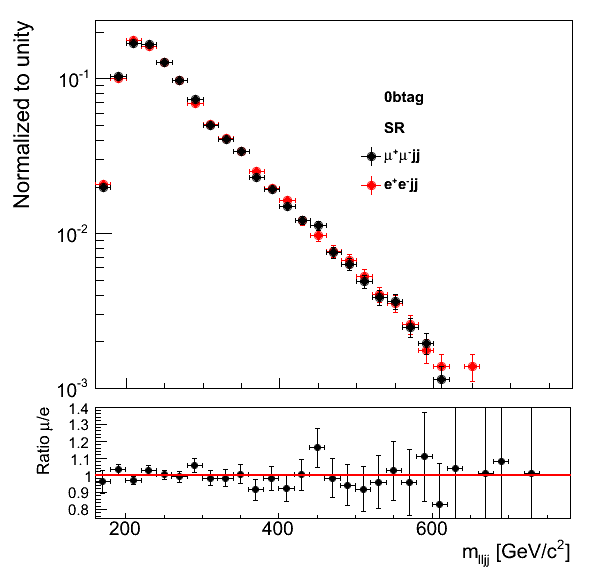
\includegraphics[width=0.33\textwidth]{plots/mH_lim20_0btag_NORM_LOG.png}
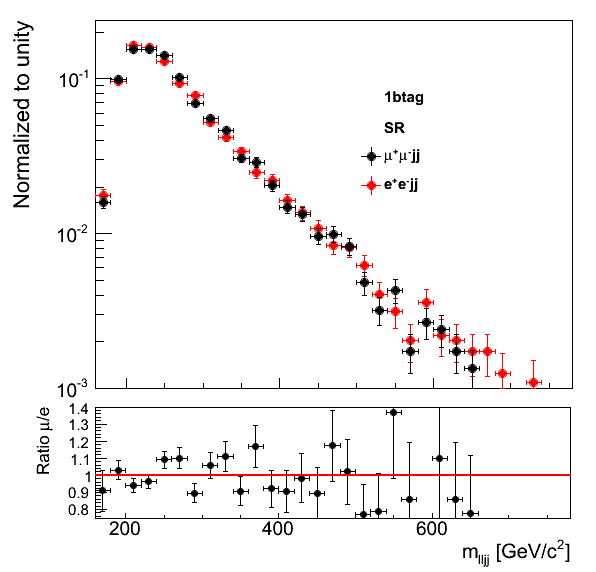
\includegraphics[width=0.33\textwidth]{plots/mH_lim20_1btag_NORM_LOG.png}
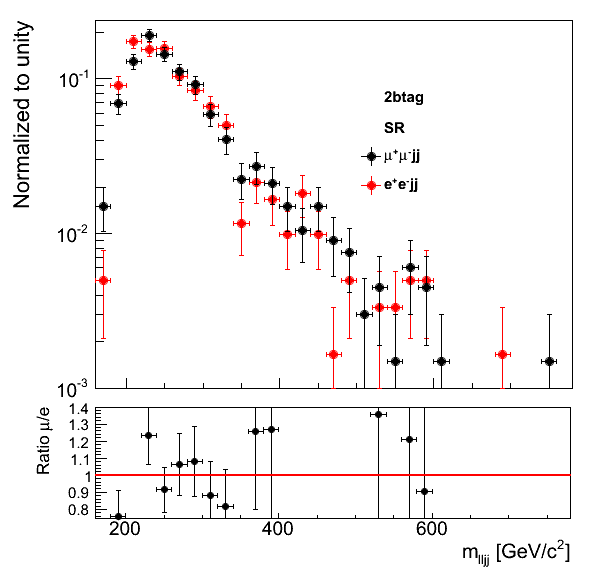
\includegraphics[width=0.33\textwidth]{plots/mH_lim20_2btag_NORM_LOG.png}
}
\centerline{
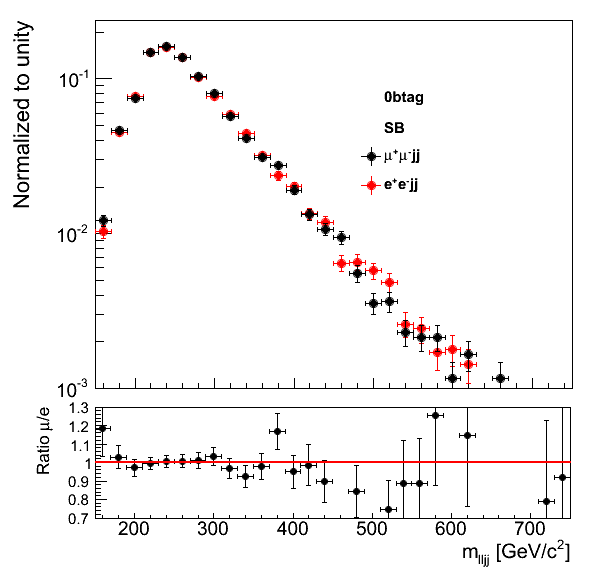
\includegraphics[width=0.33\textwidth]{plots/mH_lim20_0btag-SB_NORM_LOG.png}
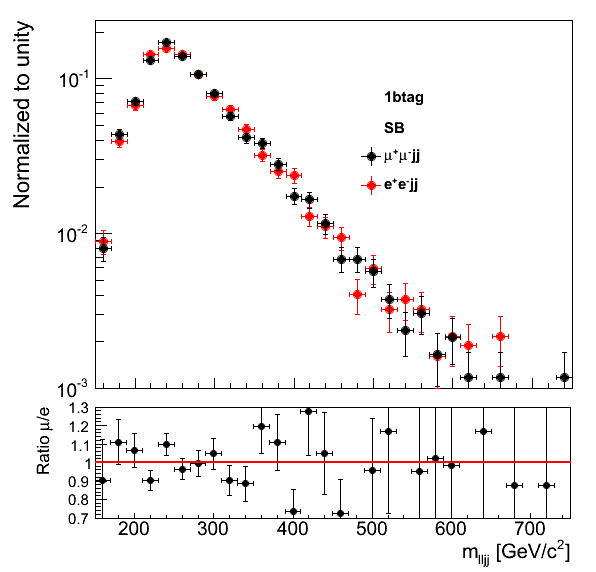
\includegraphics[width=0.33\textwidth]{plots/mH_lim20_1btag-SB_NORM_LOG.png}
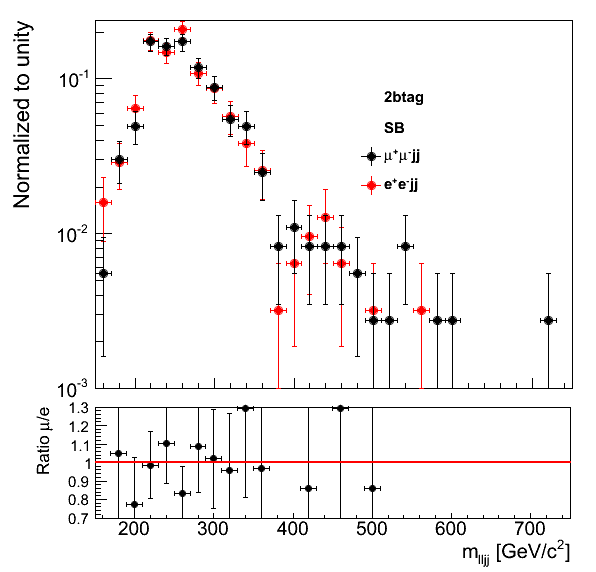
\includegraphics[width=0.33\textwidth]{plots/mH_lim20_2btag-SB_NORM_LOG.png}
}
\caption{Mass distributions of the $\LL jj$ system for events in the electron and muon channels: data in the $m_{jj}$ (top) signal and (bottom) sideband regions. From left to right, plots correspond to the 0-, 1-, and 2-btag categories.
}
\label{fig:emuratios}
\end{center}
\end{figure}

In order to minimize systematic uncertainties from Monte Carlo predictions, we normalize background to sidebands. For completeness, the signal region is 71 $< m_{jj} <$ 111 GeV and the sideband region is 60 $< m_{jj} <$ 71 GeV plus 111 $< m_{jj} <$ 130 GeV. The procedure is applied independently in each b-tag category since background composition varies between categories. The dominant backgrounds include Z+jets with either light or heavy flavor jets, and top background. These backgrounds equally populate the $m_{jj}$ signal region and $m_{jj}$ sidebands~\cite{AN-11-388}.
%The di-boson background amounts to less than 5\% in the 0 and 1 b-tag categories and about 10\% in the 2 b-tag category. A very conservative uncertainty of 30\% on Monte Carlo prediction of the di-boson production would result in only 1-3\% uncorrelated contribution to the total background prediction error. Therefore, we have developed a procedure which extrapolates the $m_{jj}$ sideband distribution of background to the signal $m_{jj}$ region. This extrapolation accounts for the 5-10\% contribution of di-boson production not modeled in sideband using Monte Carlo prediction. Uncertainties in this procedure result in uncertainties in both normalization and shape parameterization of the $m_{ZZ}$ distributions. 
If we were to rely on Monte Carlo prediction of background, uncertainties in the b-tag efficiency alone would result in about 20\% uncertainty in the 2 b-tag category. We observe good agreement of the $m_{jj}$ distributions in the three b-tag categories and in different $m_{ZZ}$ mass ranges for the range 60 $< m_{jj} <$ 130 GeV. A more detailed look at the sidebands can be seen in Section~\ref{sec:upandlowersideband}.

We can use parameterization of the $m_{ZZ}$ mass spectrum in the background Monte Carlo in the $m_{jj}$ signal region and $m_{jj}$ sideband. We create a ratio $\alpha (m_{ZZ})$ between the two, which predicts how sideband data can be scaled to obtain background prediction in the signal region. Then background expectation $N_{bkg}$ ($m_{ZZ}$) is obtained from the distribution of events in the sideband $N_{sb}$ ($m_{ZZ}$) as shown in equation~\ref{eq:alpha}.

\begin{equation} N_{bkg}(m_{ZZ}) = N_{sb}(m_{ZZ}) \times \dfrac{N_{bkg}^{MC}(m_{ZZ})}{N_{sb}^{MC}(m_{ZZ})} = N_{sb}(m_{ZZ}) \times \alpha (m_{ZZ})      \label{eq:alpha}\end{equation} \vspace {.001em}



The advantage of the above approach is that most systematic uncertainties cancel in the ratios.  The remaining factor, $\alpha$($m_{ZZ}$), reflects small kinematic differences between the signal region and sideband. This procedure also provides automatic normalization of background and makes any needed adjustments to the shape of the $m_{ZZ}$ mass spectrum. Even though we use these corrections there is very good agreement between data and Monte Carlo prediction of the $m_{ZZ}$ and $m_{jj}$ distributions after the preselection requirements~\cite{CMS-AN-HIG-13-064}.

To estimate the shape of background in data, the events in the sideband region have been scaled according to $\alpha$($m_{ZZ}$). These distributions are then fit using a parameterization derived from Monte Carlo. The fit function is a Crystal-Ball function multiplied by the Fermi-function~\cite{CrystalBall}~\cite{FermiFunction}.  The Fermi-function helps to describe the sharp kinematic turn-on at low mass, but otherwise this is a purely empirical fit. Only the width of the Gaussian core of the Crystal-Ball and the turn-over point to the power-law are free parameters in the fit. The other parameters are fixed to values extracted from the simulation~\cite{AN-11-388}. 
%The final fit result are expressed not as function of the the CB witdth and turn-over point directly, but as linear combinations of the two, such that the two resulting free parameters are uncorelated and have a mean of zero with s standard deviation of one. This is done for two reasons: (1) the current version of Higgs combination tools does not allow correlations different from $\pm$100\% or zero, so that this manual decorrelation is necessary for accurate uncertainty estimates (2) it allows for the proper inclusion of the statistical uncertainties originating from the limited Monte Carlo sample used to compute $\alpha$.
